\documentclass[sigconf,nonacm]{acmart}

\newcommand{\NOx}{NO$_x$}
\newcommand{\modelname}{PlumeWatch}

\title{Detecting Power Plant \texorpdfstring{\NOx}{NOx} Emissions Changes using
Physics-Guided Deep Learning and TEMPO Satellite Imagery}

\author{Pranav Walimbe}
\affiliation{%
  \institution{University of California, Berkeley}
  \city{Berkeley}
  \state{California}
  \country{USA}
}
\email{pranav.walimbe@berkeley.edu}

\author{Hikari Murayama}
\affiliation{%
  \institution{University of California, Berkeley}
  \city{Berkeley}
  \state{California}
  \country{USA}
}
\email{hikari\_murayama@berkeley.edu}

\author{Ron Cohen}
\affiliation{%
  \institution{University of California, Berkeley}
  \city{Berkeley}
  \state{California}
  \country{USA}
}
\email{rccohen@berkeley.edu}

\date{October 8, 2026}

\begin{document}

\begin{abstract}
NASA's Tropospheric Emissions: Monitoring of Pollution (TEMPO) instrument
provides hourly daytime observations of tropospheric nitrogen dioxide
(NO$_2$) across North America. These observations could support independent,
facility-level monitoring of power plant nitrogen oxides (\NOx{}) emissions,
filling gaps caused by continuous emissions monitoring system (CEMS) failures
and facilities not subject to hourly emissions-reporting requirements.
Previous studies have estimated hourly point-source emissions
using empirical methods, which are highly are sensitive to instrument
retrieval uncertainty, changing atmospheric conditions, TEMPO's coarse spatial
resolution, signals from nearby emission sources, and temporal mismatch with hourly
CEMS records. We instead formulate facility monitoring as change detection over
sequences of TEMPO observations. This allows the model to learn relative emissions behavior rather
than estimate exact emissions from noisy data. We develop a convolutional gated recurrent unit (ConvGRU) model that processes five consecutive TEMPO observations
together with meteorological, plume-transport, and tabular features encoding time of day and seasonality to
classify power plant emission trajectories as increasing, steady, or decreasing
On a held-out evaluation set containing more than 20,000 samples from over 95 U.S. power
plants observed between August 2023 and July 2026, the ConvGRU model achieved a
classification Macro-F1 score of 0.56, which outperformed a baseline Multilayer Perceptron (MLP) trained only on the same time-derived features and scoring 0.45.
Our findings suggest that our ConvGRU model can identify power plant emissions signals
from TEMPO observations beyond the time-derived features shared with the baseline MLP. More broadly, they indicate
that change detection may offer a more tractable framework for modeling power plant activity from TEMPO observations
compared to estimating absolute emissions.
\end{abstract}

\maketitle

\section{Introduction}

Based on U.S. Environmental Protection Agency (EPA) inventory data, power plants
in the U.S. electricity-generation sector emitted approximately 0.74 million
short tons of \NOx{} in 2023, about 9.5\% of national
emissions~\cite{epa2026emissionsTrends}. \NOx{} emissions contribute to
ground-level ozone and secondary particulate matter, pollutants that can
inflame and damage the airways, reduce lung function, and aggravate
asthma~\cite{epa2016noxHealth}. EPA regulations require most large U.S.
fossil-fuel-fired generating units that produce electricity for sale to submit
unit-level hourly emissions data on a quarterly basis~\cite{epa2026powerMonitoring}.
However, monitoring equipment malfunctions and maintenance can make CEMS
measurements unavailable or invalid, requiring plants to report calculated
substitute values instead of direct measurements~\cite{epa2021substitute}.
Behind-the-meter generators that do not sell electricity can fall outside
federal hourly reporting requirements, such as the natural gas
turbines powering SpaceXAI's Colossus 2 data center~\cite{gauld2026dataCenter}.
Outside the United States, comparable public, hourly, unit-level emissions data are generally unavailable;
global inventories typically provide only annual estimates~\cite{huang2026detectability}. Independent estimates could therefore
fill reporting gaps and provide timely insight into facility operations ahead of the EPA's quarterly release
of hourly emissions data.

TEMPO is an ultraviolet-visible spectrometer hosted aboard a geostationary satellite
that observes tropospheric vertical column densities (TVCDs) for various trace gases
across North America during daylight hours~\cite{zoogman2017tempo}. Earlier polar-orbiting
instruments, including the Ozone Monitoring Instrument (OMI) and TROPOspheric Monitoring
Instrument (TROPOMI), typically observe a given location once per day; TEMPO's geostationary
view provides approximately hourly scans with finer spatial
resolution~\cite{levelt2006omi,veefkind2012tropomi,zoogman2017tempo}. Hourly sampling
captures intraday changes in emissions plumes and atmospheric transport that daily
observations can miss. However, power plant emissions signals in TEMPO NO$_2$ TVCDs can be weakened
or obscured by factors including evolving meteorology and atmospheric chemistry, cloud cover,
viewing geometry and retrieval uncertainty, dilution within TEMPO's \(2.0~\mathrm{km} \times 4.75~\mathrm{km}\) spatial resolution, and interference from nearby emission sources~\cite{tempo2026userGuide,huang2026detectability,gauld2026dataCenter}.
Cross-comparisons with CEMS data, which is the most reliable ground truth available, introduce an
additional temporal mismatch because TEMPO observes a facility at a specific time during each hourly scan,
whereas CEMS data aggregate emissions over an entire clock hour~\cite{tempo2026userGuide,epa2026powerMonitoring}.

Satellite instruments measure atmospheric column abundance rather than emissions
directly. Lightweight inversion methods therefore infer source rates from the
spatial structure of an observed plume and estimated winds. Cross-sectional flux
(CSF) removes the background column, integrates the remaining enhancement across
transects perpendicular to the plume, and multiplies the resulting line density by
an effective wind speed. Under steady-state conditions, this flux approximates the
source emission rate. The directional derivative approach (DDA) instead combines
the wind field with spatial gradients in the observed column to estimate a local
source term, which is then integrated around the
facility~\cite{santaren2025benchmarking,sun2025hourly}.

Although promising, these methods have not performed consistently across source
strengths and observing conditions. In synthetic satellite scenes with realistic
cloud filtering and reanalysis winds, Santaren et al. reported annual relative
RMSEs of 20\% for Gaussian plume inversion, 27\% for CSF, and 31\% for lightweight
CSF~\cite{santaren2025benchmarking}. Cloud filtering disproportionately reduced
wintertime coverage and prevented the methods from reliably reproducing
month-to-month emission variability. With TEMPO observations, Sun et al. improved
correlations with CEMS at 10 of 14 power plants by incorporating changes between
consecutive NO$_2$ columns, although the resulting estimates remained approximately
fourfold lower than CEMS measurements~\cite{sun2025hourly}. Beaudry et al. used a
rise--decay model that separately fits near-source NO$_2$ buildup and downwind plume
decay, estimating average emissions within 50\% of CEMS values at 27 of 64 plants
but exhibiting substantially greater bias below
\(250~\mathrm{kg~NO_2~h^{-1}}\)~\cite{beaudry2026quantification}.

Machine learning (ML) studies have addressed several related point-source monitoring
tasks. Huang and Wang trained a tabular MLP to predict whether a TROPOMI observation
contained a detectable power-plant NO$_2$ plume using 25 facility, meteorological,
surface, and sensor variables sampled at the plant location~\cite{huang2026detectability}.
Their models achieved F1 scores above 0.66, but detectability
ranged from below 20\% to above 60\% for plants with similar emissions. Their
interference filters also retained plants representing only 45.0\% of U.S. and 21.1\%
of global NO$_x$ emissions in their datasets. Alnaim et al. used stacked long
short-term memory (LSTM) networks to predict next-day EPA-reported NO$_2$ emissions from seven-day sequences of previous
emissions, scalar TROPOMI observations, MERRA-2 meteorology, aerosol measurements,
and calendar variables~\cite{alnaim2022evaluating}. Their best single-plant LSTM
retained an error near 40\%, while multi-plant experiments exceeded 55\% error and
often underestimated extreme values. Dumont et al. trained CNNs to estimate
power-plant CO$_2$ emissions from simulated XCO$_2$ and wind fields, with optional
NO$_2$ inputs, and obtained median relative errors of approximately 20--25\% at
geographically held-out plants~\cite{dumont2024deepLearning}. Their evaluation used
synthetic scenes that did not represent clouds or structured satellite-retrieval
errors.

The point-source ML studies reviewed above do not jointly model the spatial
structure and temporal evolution of consecutive trace-gas satellite rasters. We instead formulate
facility monitoring as change detection over five TEMPO scans. Classifying
emissions as increasing, steady, or decreasing preserves information about
short-term facility behavior while reducing reliance on recovering exact emissions amounts from noisy observations.

Two relevant model families are convolutional recurrent neural networks
(CRNNs) and spatiotemporal vision transformers (ViTs). At each timestep, a CRNN
combines features from the current raster with a spatially structured state
carried from the preceding timestep. Convolutional operations within the
recurrent cell preserve the raster grid and update each location using its
surrounding neighborhood. ConvLSTM controls separate cell and hidden states
through input, forget, and output gates, providing explicit control over memory
retention at the cost of additional parameters and computation. ConvGRU instead
maintains one hidden state controlled by reset and update gates, producing a
more compact recurrent model with less explicit control over long-term
memory~\cite{shi2015convlstm,ballas2015convgru}. Spatiotemporal ViTs divide each
raster into patches and use self-attention to connect patch representations
across locations and timesteps. This provides direct access to global
space--time relationships without recurrent processing, but supplies a weaker
locality bias and shifts more pattern learning to the training data; the
computational cost also grows with the number of patches and
timesteps~\cite{bertasius2021timesformer}.

We select ConvGRU to balance modeling capacity with parameter efficiency. Each
sample spans only five scans, so ConvLSTM's additional memory state offers less
apparent benefit than it would for longer sequences while increasing the number
of model parameters. The input rasters are also small ($24 \times 24$ pixels),
and power plant plumes generally form connected clusters of pixels whose evolution
can be captured through local convolutional operations rather than
long-range interactions. Also, TEMPO only has roughly three years of observations available
while limits our overall dataset size. A compact ConvGRU therefore provides spatial memory without the added complexity
of ConvLSTM or a spatiotemporal ViT.

\section{Data Sources}

\subsection{TEMPO NO\texorpdfstring{$_2$}{2} Data}

NASA distributes TEMPO NO$_2$ retrievals in two formats: Level 2 data on the
instrument's native measurement footprints and Level 3 data regridded from each
east-to-west scan~\cite{tempo2026userGuide}. We downloaded version 4 Level 2
NO$_2$ retrievals from August 2023 through August 2026. Along with NO$_2$
TVCDs, the product provides metadata including native footprint geometry,
mirror-step observation times, main data quality flags, and effective cloud
fractions, which we later use for regridding, quality filtering, and temporal
alignment with CEMS records.

\subsection{CEMS Records}

We downloaded hourly emissions records for individual power plant units and
annual facility and unit attributes from the U.S. Environmental Protection
Agency's Clean Air Markets Program Data (CAMPD) APIs for August 2023 through
September 2026. From the hourly records, we use facility and unit identifiers,
reporting date and hour, \NOx{} mass and its measurement flag, and operating time.
From the annual attributes, we use facility coordinates.

\subsection{HRRR Weather Data}

The High-Resolution Rapid Refresh (HRRR) is an hourly weather model with a
3~km grid covering the contiguous United States. From NOAA's public HRRR
archive, we downloaded hourly 2~m air temperature and eastward and northward
wind components at 80~m above ground for August 2023 through August 2026.

\section{Methods}

\subsection{AOI Construction}

For each power plant, we define a 72~km $\times$ 72~km area of interest (AOI)
centered on the facility and divide it into a $24 \times 24$ grid of
3~km $\times$ 3~km cells. For each AOI-hour, we sum the unit-level \NOx{} mass
reported by all facilities in the AOI and discard the hour if any contributing
measurement is invalid or unavailable. We score each AOI using its median total
\NOx{} mass across hours whose mean unit operating time meets or exceeds the
AOI-specific median. We retain the highest-scoring 50\% to focus the dataset on
emissions signals more likely to be detected by TEMPO.

\subsection{TEMPO Regridding and Quality Filtering}

TEMPO Level 2 observations lie on irregular native footprints, whereas our
model uses a fixed spatial grid. We project the footprint boundaries and AOI
grid to the contiguous-U.S. Albers equal-area coordinate system. We then assign
each AOI grid cell an NO$_2$ TVCD by averaging the TEMPO footprints that
intersect it, weighted by their area of overlap. Figure~\ref{fig:tempoRegridding}
illustrates this mapping from native footprints to the fixed AOI grid.

\begin{figure}[t]
    \centering
    \IfFileExists{visuals/tempo-regridding.pdf}{%
        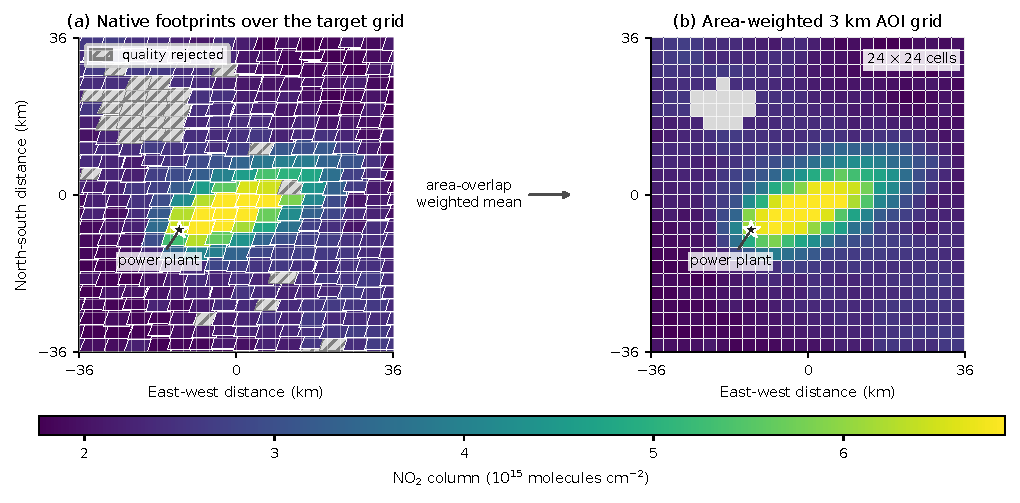
\includegraphics[width=0.96\columnwidth]{visuals/tempo-regridding.pdf}%
    }{%
        \fbox{\parbox[c][1.15in][c]{0.91\columnwidth}{\centering
        Regridding schematic placeholder}}}
    \caption{TEMPO Level 2 regridding to the AOI grid.}
    \Description{TEMPO footprints mapped to the AOI grid.}
    \label{fig:tempoRegridding}
    \vspace{-0.8\baselineskip}
\end{figure}

A footprint contributes to the NO$_2$ average only when a given pixel's main data quality
flag equals zero (TEMPO metadata that indicates reliable retrievals) and its effective cloud fraction does not exceed 0.20. Grid
cells without an accepted footprint overlap remain masked, and we retain a
binary mask of the original valid cells. We use bilinear interpolation to fill
masked NO$_2$ pixels for downstream modeling.

\subsection{Sample Construction}

Each sample contains five consecutive observations of one AOI, indexed from
$t_0$ to $t_4$. We retain a sequence only when each pair of adjacent TEMPO
scans is separated by 40--70 minutes and every NO$_2$ raster has valid pixel coverage of at
least 85\%. At each timestep, we pair the TEMPO raster with
the HRRR temperature and wind rasters from the closest hour interpolated to the same
$24 \times 24$ raster size and spatial coverage as the NO$_2$ rasters.

Because CEMS records correspond to clock hours rather than TEMPO scan times,
we linearly interpolate the AOI-hour \NOx{} emissions between the surrounding
hourly CEMS records at each scan time. Let $E_i$ denote the interpolated emissions
at time $t_i$. For scans $t_a$ through $t_b$, we calculate the time-weighted mean
\begin{equation}
    \overline{E}_{a:b} =
    \frac{\sum_{i=a}^{b-1}(t_{i+1}-t_i)(E_i+E_{i+1})/2}
    {t_b-t_a}.
\end{equation}
We define the sequence change as
$\Delta E=\overline{E}_{2:4}-\overline{E}_{0:2}$ and use the threshold
$\theta=250~\mathrm{lb\,h^{-1}}$ to assign its category:
\begin{equation}
    c =
    \begin{cases}
        \text{increase}, & \Delta E \geq \theta, \\
        \text{steady}, & -\theta < \Delta E < \theta, \\
        \text{decrease}, & \Delta E \leq -\theta.
    \end{cases}
\end{equation}

Figure~\ref{fig:sample-construction} shows one complete five-timestep model
input and its derived behavior label.

\begin{figure*}[t]
  \centering
  \IfFileExists{visuals/sample-construction.pdf}{%
      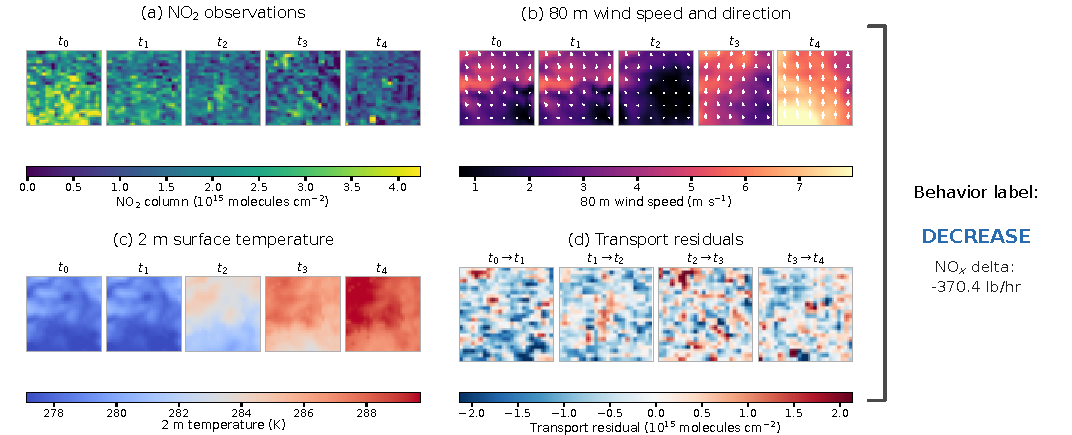
\includegraphics[width=\textwidth]{visuals/sample-construction.pdf}%
  }{%
      \fbox{\parbox[c][2.9in][c]{0.95\textwidth}{\centering
      \textit{Placeholder: complete five-timestep raster inputs, transport residuals,}\\[0.25em]
      \textit{and emissions-change behavior label}}}
  }
  \caption{Complete model inputs and behavior label for one five-timestep training sample.}
  \Description{Five NO2, wind, and temperature rasters, four transport residuals,
  and the associated emissions-change behavior label.}
  \label{fig:sample-construction}
\end{figure*}

\subsection{Transport Model}

Emissions change signal in consecutive NO$_2$ rasters can be degraded by
movement and decay of the existing plume. For each adjacent
pair, we use a simple transport model to predict the next NO$_2$ observation without new emissions in the AOI.
We then subtract this prediction from the observed next raster to obtain a
transport residual, which separates plume structure explained by modeled
advection, horizontal dispersion, and chemical decay from remaining variation that may
reflect emissions changes within the AOI.

For the interval $\Delta t_i=t_{i+1}-t_i$, let $N_i(\boldsymbol{x})$ and
$N_{i+1}(\boldsymbol{x})$ denote the earlier and later NO$_2$ rasters,
$\boldsymbol{u}_i(\boldsymbol{x})$ and
$\boldsymbol{u}_{i+1}(\boldsymbol{x})$ their wind fields, and $B_i$ the median
NO$_2$ value along the boundary of the earlier raster.

\begingroup
\makeatletter
\tagsleft@true
\makeatother
\begin{align}
  \overline{\boldsymbol{u}}_i
    &= \gamma\!\left[(1-\lambda)\boldsymbol{u}_i
       + \lambda\boldsymbol{u}_{i+1}\right]
       \tag{i}\label{eq:transport-wind} \\
  A_i(\boldsymbol{x})
    &= N_i\!\left(\boldsymbol{x}
       -\overline{\boldsymbol{u}}_i(\boldsymbol{x})\Delta t_i\right)
       \tag{ii}\label{eq:transport-advection} \\
  \sigma_i
    &= \sigma_0\sqrt{\frac{\Delta t_i}{1~\mathrm{h}}}
       \tag{iii}\label{eq:transport-diffusion-scale} \\
  D_i
    &= B_i+G_{\sigma_i}*(A_i-B_i)
       \tag{iv}\label{eq:transport-diffusion} \\
  \widehat{N}_{i+1}
    &= B_i+\exp\!\left(-\frac{\Delta t_i}{\tau}\right)(D_i-B_i)
       \tag{v}\label{eq:transport-decay} \\
  R_i
    &= N_{i+1}-\widehat{N}_{i+1}
       \tag{vi}\label{eq:transport-residual}.
\end{align}
\endgroup

Equations~\eqref{eq:transport-wind} and
\eqref{eq:transport-advection} represent wind-driven advection. Satellite
columns do not resolve the vertical distribution of plume mass, so
point-source methods commonly use an effective wind to approximate its mean
transport speed~\cite{santaren2025benchmarking,meier2024conversion}. We
approximate this wind by averaging the fields at the two endpoints
($\lambda=0.5$) and applying a modest speed correction ($\gamma=0.8$).
Equation~\eqref{eq:transport-advection} then applies semi-Lagrangian advection
by tracing each destination cell backward along the effective wind over
$\Delta t_i$ and bilinearly sampling the earlier raster at the resulting
departure location.

Equations~\eqref{eq:transport-diffusion-scale} and
\eqref{eq:transport-diffusion} approximate unresolved turbulent horizontal
dispersion. Gaussian plume representations are widely used in satellite
point-source studies~\cite{santaren2025benchmarking,meier2024conversion}. We
set $\sigma_0$ to one 3~km grid cell after one hour and increase the width with
$\sqrt{\Delta t_i}$. Applying the Gaussian
kernel to $A_i-B_i$ spreads the plume enhancement while preserving the
estimated background.

Equation~\eqref{eq:transport-decay} applies first-order loss to the
above-background enhancement. The effective timescale $\tau=8$~h represents
the combined persistence of the observed NO$_2$ plume under chemical removal
and other unresolved losses. Exponential loss is commonly used to describe the downwind decay of
satellite-observed NO$_x$ plumes, whose effective lifetimes vary with
meteorology and plume chemistry~\cite{meier2024conversion}.
Equation~\eqref{eq:transport-residual} subtracts the resulting transport-only
prediction from the next observation.

Each five-observation sample yields four residual rasters. We apply the same
advection and diffusion operations to the earlier validity mask and combine it
with the later mask to produce quality masks for the transport residuals. The transport-residual panel in
Figure~\ref{fig:sample-construction} shows the four adjacent-scan residuals for
the same example sequence.

\subsection{Dataset Stratification}

Our split design has three goals: prevent leakage from overlapping AOIs,
approximate a 70\%/15\%/15\% division, and construct class distributions that
support balanced training and comparable evaluation across the held-out
splits. We group overlapping AOIs into connected clusters and treat each
cluster as an indivisible assignment unit. Because each cluster contains an
arbitrary number of AOIs, samples, and class instances, cluster-level
assignment cannot generally meet every target exactly.

We use mixed-integer linear programming (MILP) to assign each geographic
cluster to exactly one split while minimizing normalized deviations from
target AOI and eligible-sample counts. The first optimization targets a
70\%/15\%/15\% train--validation--test division using AOI and sample counts,
after which we fix the training clusters. A second optimization assigns the
remaining clusters equally between validation and test while balancing AOI,
sample, and per-class counts. It also constrains both held-out splits to have
the same median number of plant units per AOI as the combined held-out pool.

We then uniformly downsample each training class to the size of the smallest
class. In validation and test, we retain every increase and decrease sample and
uniformly subsample steady samples to at most the size of the larger change
class. Subsequent raster-quality filtering can alter the final class counts,
and we do not rebalance the surviving samples.

\subsection{ConvGRU Model}

Our ConvGRU model separately encodes five observation frames and four transport residuals,
integrates their spatial feature maps across
the sequence, and fuses the final recurrent representation with temporal
features to classify emissions behavior. Figure~\ref{fig:convgru-architecture}
summarizes the complete architecture and the operations within one ConvGRU
cell.

\begin{figure*}[t]
  \centering
  \IfFileExists{visuals/convgru-architecture.pdf}{%
      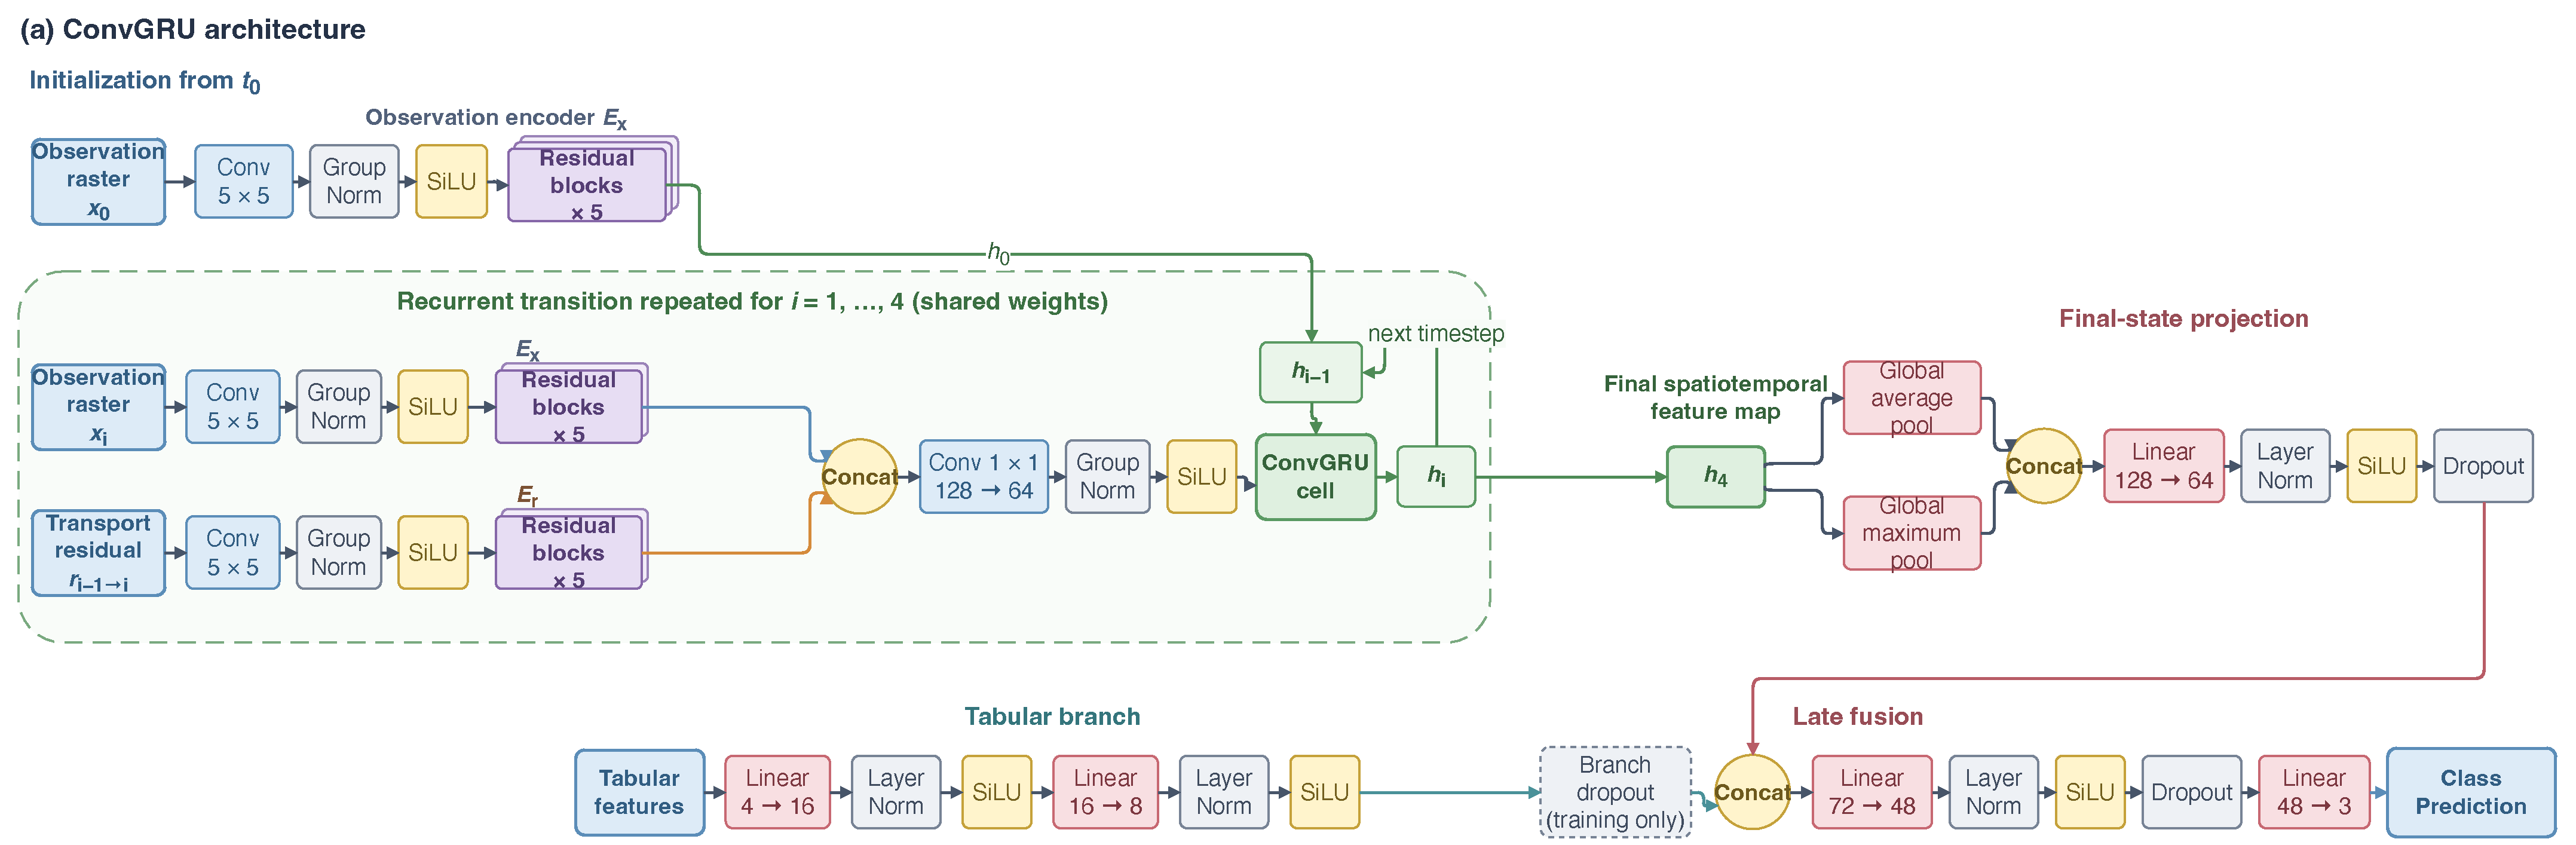
\includegraphics[width=0.96\textwidth]{visuals/convgru-architecture.pdf}%
  }{%
      \fbox{\parbox[c][1.35in][c]{0.93\textwidth}{\centering
      \textbf{(a) Overall architecture placeholder}\\[0.35em]
      Observation and residual encoders $\rightarrow$ ConvGRU sequence
      $\rightarrow$ visual pooling $\rightarrow$ late fusion $\rightarrow$
      behavior class}}
  }

  \vspace{0.55em}

  \IfFileExists{visuals/convgru-cell.pdf}{%
      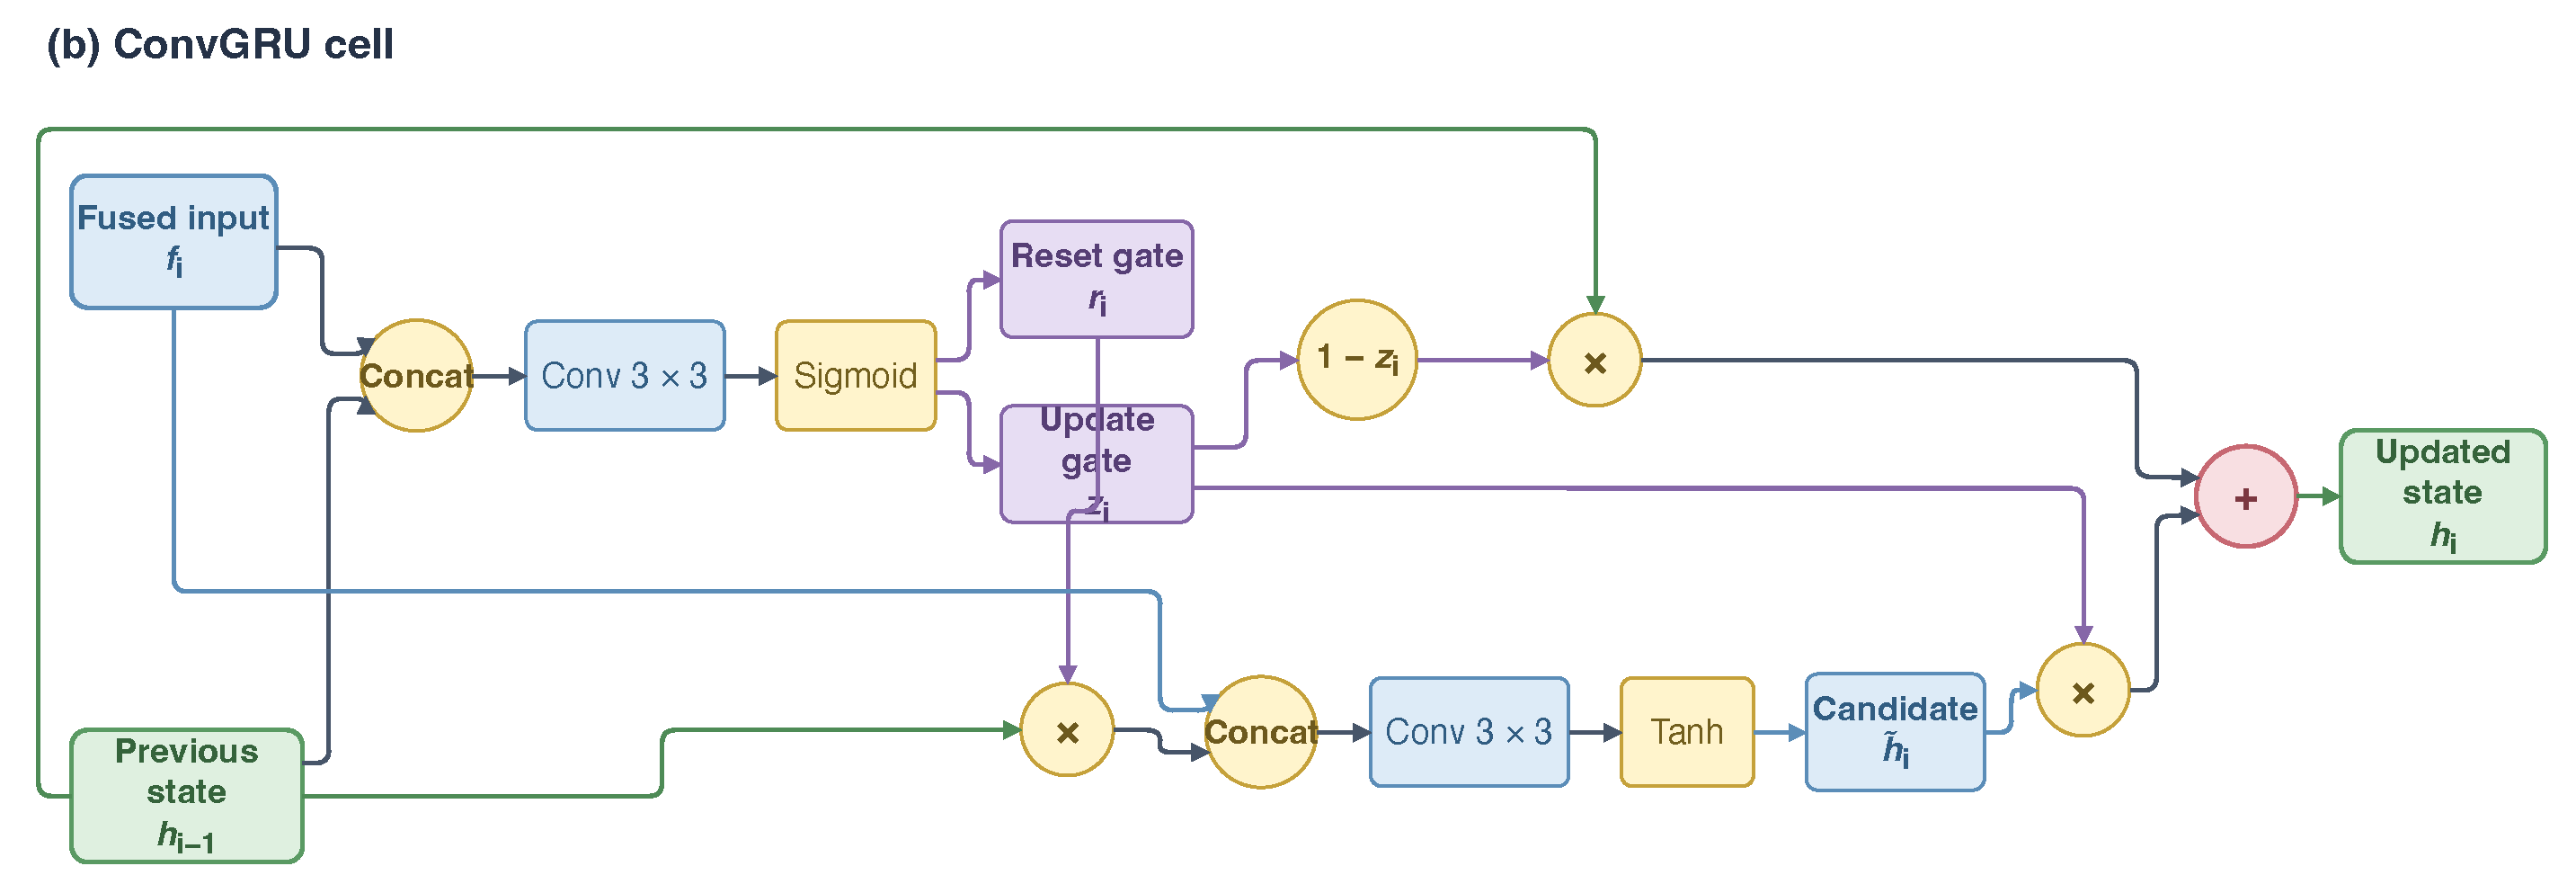
\includegraphics[width=0.55\textwidth]{visuals/convgru-cell.pdf}%
  }{%
      \fbox{\parbox[c][0.92in][c]{0.53\textwidth}{\centering
      \textbf{(b) ConvGRU cell placeholder}\\[0.3em]
      Reset gate, update gate, candidate state, and hidden-state update}}
  }
  \caption{ConvGRU model. (a) Complete raster-encoding, recurrent-integration,
  and classification workflow. (b) Operations within one ConvGRU cell.}
  \Description{Two-panel placeholder for the complete ConvGRU architecture and
  the reset, update, candidate, and hidden-state operations within one cell.}
  \label{fig:convgru-architecture}
\end{figure*}

Each observation frame contains five channels: NO$_2$, its quality mask, the
eastward and northward 80~m wind components, and 2~m temperature. Each
transport-residual frame contains the residual and its quality mask. Separate
observation and residual encoders account for the different meanings of these
inputs, while each encoder shares its weights across all frames in its branch.
Both encoders begin with a $5\times5$ convolution that produces 32 channels,
followed by five residual blocks. Strided blocks increase the channel width
from 32 to 48 and then 64 while reducing each $24\times24$ raster to a
$64\times6\times6$ feature map. The frame encoders use group normalization and
SiLU activations.

As shown in Figure~\ref{fig:convgru-architecture}(a), the encoded $t_0$
observation initializes the hidden state, so the model does not synthesize a
residual before the first observation. At each subsequent timestep $t_i$, the
model concatenates the encoded observation with the encoded residual for
$t_{i-1}\rightarrow t_i$. A $1\times1$ convolution, group normalization, and
SiLU activation reduce the resulting 128 channels to the 64-channel input for
the recurrent cell.

Figure~\ref{fig:convgru-architecture}(b) expands one recurrent update. Let
$\boldsymbol{f}_i$ denote the fused input and $\boldsymbol{h}_{i-1}$ the
previous hidden state. The ConvGRU computes
\begin{align}
  [\boldsymbol{r}_i,\boldsymbol{z}_i]
    &= \sigma\!\left(W_g *
       [\boldsymbol{f}_i,\boldsymbol{h}_{i-1}]+\boldsymbol{b}_g\right), \\
  \widetilde{\boldsymbol{h}}_i
    &= \tanh\!\left(W_h *
       [\boldsymbol{f}_i,\boldsymbol{r}_i\odot\boldsymbol{h}_{i-1}]
       +\boldsymbol{b}_h\right), \\
  \boldsymbol{h}_i
    &= (1-\boldsymbol{z}_i)\odot\boldsymbol{h}_{i-1}
       +\boldsymbol{z}_i\odot\widetilde{\boldsymbol{h}}_i,
\end{align}
where $[\cdot,\cdot]$ denotes channel-wise concatenation and $*$ denotes a
$3\times3$ convolution. The reset gate
$\boldsymbol{r}_i$ controls how much previous spatial information contributes
to the candidate state, while the update gate $\boldsymbol{z}_i$ determines
how much of that candidate replaces the previous state.

After the fourth recurrent update, global average and maximum pooling each
reduce the final $64\times6\times6$ state to 64 values. Average pooling
summarizes distributed spatial evidence, while maximum pooling retains strong
localized responses. The model concatenates both outputs and projects the
result to a 64-dimensional visual embedding using layer normalization and a
SiLU activation. A separate feedforward encoder
maps the four time-derived tabular features from 4 to 16 and then 8 dimensions. We
concatenate this tabular embedding with the visual embedding only after
recurrent processing, producing the 72-dimensional input to a
$72\rightarrow48\rightarrow3$ classification head. Its 48-unit hidden layer
uses layer normalization and a SiLU activation before the linear output layer.

\subsection{Baseline MLP Model}

We use a lightweight baseline MLP with time-derived features to gauge how much emissions-change
behavior can be predicted from recurring daily and annual patterns without
satellite or weather inputs. We represent each sample using
four cyclic features: the sine and cosine of local solar hour (midpoint of timesteps) and the sine and
cosine of day of year. The baseline MLP maps these features through hidden layers of 16
and 8 units, each followed by layer normalization and a SiLU activation. A
linear output layer produces logits for the three behavior classes.

\subsection{Training Procedure}

Table~\ref{tab:dataset-composition} summarizes the final dataset used to train
and evaluate both models. We standardize the NO$_2$, wind, temperature, and
transport residual rasters and the tabular inputs using the corresponding
training set mean and standard deviation across all splits.

\begin{table}[t]
  \caption{Dataset composition by split and class.}
  \label{tab:dataset-composition}
  \centering
  \small
  \begin{tabular}{@{}lrrrrr@{}}
    \toprule
    Split & AOIs & Decrease & Steady & Increase & Total \\
    \midrule
    Training   & 469 & 17,130 & 23,289 & 29,888 & 70,307 \\
    Validation & 101 & 3,198 & 8,589 & 10,411 & 22,198 \\
    Test       & 97 & 3,184 & 7,764 & 10,093 & 21,041 \\
    \bottomrule
  \end{tabular}
\end{table}

\begin{table}[t]
  \caption{Training configuration.}
  \label{tab:training-configuration}
  \centering
  \small
  \begin{tabular}{@{}lcc@{}}
    \toprule
    Parameter & Baseline MLP & ConvGRU \\
    \midrule
    Trainable parameters & 291 & 724,939 \\
    Optimizer & \multicolumn{2}{c}{AdamW} \\
    Batch size & 128 & 128 \\
    Initial learning rate & $10^{-3}$ & $6.04 \times 10^{-5}$ \\
    Weight decay & $10^{-4}$ & $10^{-4}$ \\
    Activation dropout & -- & 0.20 \\
    Tabular branch dropout & -- & 0.25 \\
    Gradient-norm limit & \multicolumn{2}{c}{5.0} \\
    LR scheduler & \multicolumn{2}{c}{Reduce on plateau} \\
    LR reduction factor & \multicolumn{2}{c}{0.5} \\
    Scheduler patience & \multicolumn{2}{c}{5 epochs} \\
    Selection metric & \multicolumn{2}{c}{Validation macro-F1} \\
    Early-stopping patience & \multicolumn{2}{c}{10 epochs} \\
    Hardware & \multicolumn{2}{c}{1 NVIDIA RTX A5000 GPU} \\
    \bottomrule
  \end{tabular}
\end{table}

For the ConvGRU, we also apply tabular branch dropout during training: for
each sample, the tabular embedding is fully zeroed with
probability 0.25 before late fusion. This discourages the classifier from
relying on the time-derived tabular features alone.

Both classifiers use inverse-frequency class weights computed from the final
training split and minimize weighted cross-entropy.

\section{Results}

\subsection{Classification Performance}

\begin{figure*}[!t]
  \centering
  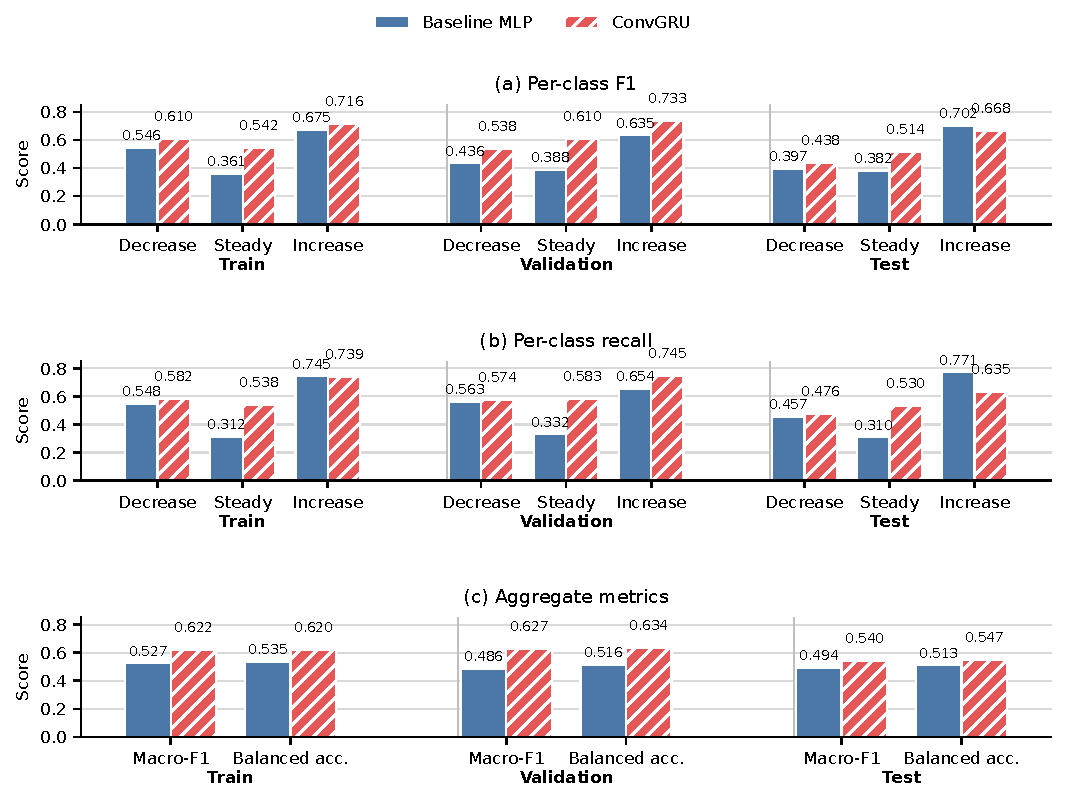
\includegraphics[width=\textwidth]{visuals/classification-performance.pdf}
  \caption{Classification performance by split.}
  \Description{Baseline MLP and ConvGRU per-class F1, per-class recall, and
  aggregate classification metrics for the training, validation, and test splits.}
  \label{fig:classification-performance}
\end{figure*}

We evaluate classification using Macro-F1 and balanced accuracy to account for class balance.
On the test set, the ConvGRU achieves a macro-F1 of 0.559 and balanced accuracy of 0.563, compared with 0.454 and 0.481
for the baseline MLP. As shown in Figure~\ref{fig:classification-performance},
the ConvGRU model demonstrates improved per-class F1 and recall scores over the baseline MLP across nearly
all per-split evaluations.

The largest performance gap between the models consistently occurs for steady samples, ranging from 0.141 to 0.143 F1 points
across splits. This makes intuitive sense because steady samples are less likely to belong to a distinct season
(e.g., increases occur more during summer, decreases occur more during winter), which means time-only features explain less plant emissions
activity for those samples. The ConvGRU model shows weakest performance on decrease samples, scoring 0.471 on decrease-only recall
for the test set, which was less than the baseline MLP that scored 0.527. The weaker performance on decrease samples may
have two causes. First, decrease events are less prevalent than increase events in the dataset, giving the model fewer
examples from which to learn. Second, after facility emissions decline, previously emitted NO$_2$ can remain visible as
the plume advects, disperses, and decays, delaying the raster response to the underlying activity change.

\subsection{Performance Across Evaluation Strata}

\subsubsection{Performance Across Months}

\begin{figure}[H]
  \centering
  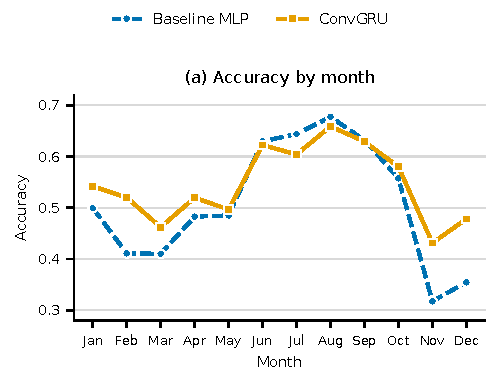
\includegraphics[width=0.86\columnwidth]{visuals/stratified-performance-monthly.pdf}
  \caption{Classification accuracy by month.}
  \Description{Baseline MLP and ConvGRU classification accuracy for each month.}
  \label{fig:stratified-performance-monthly}
\end{figure}

As shown in Figure~\ref{fig:stratified-performance-monthly}, the ConvGRU model
shows more consistent monthly accuracy than the baseline MLP. The models perform
most similarly during summer, while their accuracy gap reaches 0.277 in April
and 0.323 in November. These results are consistent with our observation that increase samples occur more during summer
and decrease samples occur more during winter. While the baseline MLP is restricted to learning seasonal patterns for
power plant activity only, the ConvGRU can use visual signal to predict emissions behavior when seasonality alone is
generally a poor indicator of activity, such as spring and fall seasons.

\subsubsection{Performance by Local Solar Hour}

\begin{figure}[H]
  \centering
  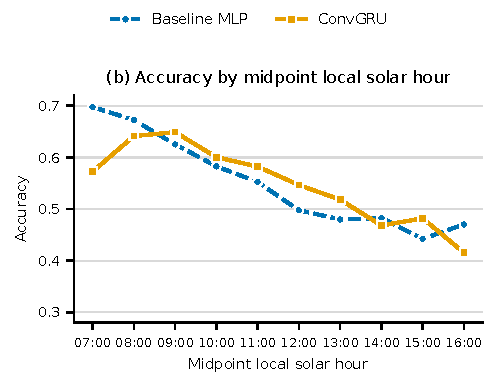
\includegraphics[width=0.86\columnwidth]{visuals/stratified-performance-solar-hour.pdf}
  \caption{Classification accuracy by midpoint local solar hour.}
  \Description{Baseline MLP and ConvGRU classification accuracy for each
  midpoint local solar hour.}
  \label{fig:stratified-performance-solar-hour}
\end{figure}

As shown in Figure~\ref{fig:stratified-performance-solar-hour}, the ConvGRU model generally demonstrates higher
accuracy at each solar hour than the baseline MLP, with both models showing a decreasing accuracy trend as local
solar hour decreases. The decreasing accuracy trend likely stems from increase samples occuring more during earlier solar hours
(which the models generally predict well) and decrease samples occuring more during the later solar hours (which the models generally
predict relatively worse).

\subsubsection{Performance by AOI Median \NOx{} Emissions}

\begin{figure}[H]
  \centering
  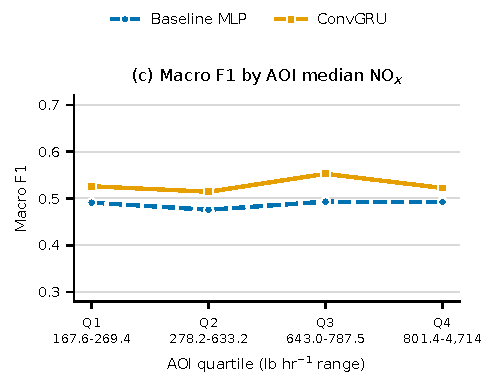
\includegraphics[width=0.86\columnwidth]{visuals/stratified-performance-aoi-nox.pdf}
  \caption{Macro-F1 by AOI median \NOx{} emissions group.}
  \Description{Baseline MLP and ConvGRU macro-F1 for AOIs in the lower and
  upper halves of median NOx emissions.}
  \label{fig:stratified-performance-aoi-nox}
\end{figure}

As shown in Figure~\ref{fig:stratified-performance-aoi-nox}, both models show a roughly equal performance improvement
when we compare Macro-F1 scores on AOIs belonging to the lower 50\% median \NOx{} of the test set versus upper
50\% median \NOx{} of the test set. This suggests that AOIs with higher-emission facilities offer better visual signal
in their raster sequences to predict ativity.

\subsubsection{Performance by Census Region}

\begin{figure}[H]
  \centering
  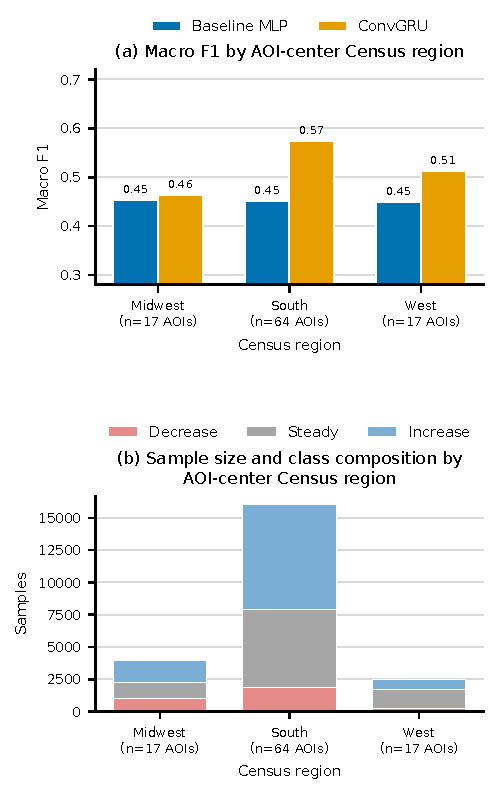
\includegraphics[width=0.86\columnwidth]{visuals/stratified-performance-census-region.pdf}
  \caption{Macro-F1 by AOI-center Census region.}
  \Description{Baseline MLP and ConvGRU macro-F1 for AOIs in the Midwest,
  South, and West Census regions.}
  \label{fig:stratified-performance-census-region}
\end{figure}

As shown in Figure~\ref{fig:stratified-performance-census-region}, the ConvGRU
gains most over the baseline MLP in the South and least in the Midwest. The
clearest observed relationship is regional class composition. Increase samples,
the ConvGRU's strongest class, comprise 50.5\% of Southern test records. The
Midwest contains the largest decrease share at 26.1\%, corresponding to the
model's weakest class, while the West is dominated by steady samples, for which
imagery provides the largest improvement over the baseline. These differences
likely contribute to the regional performance pattern.

Regional representation during training may also matter. Southern records
comprise 62.8\% of the training set, compared with 21.3\% from the Midwest and
5.1\% from the West, giving the model greater exposure to Southern facilities
and their visual characteristics. Fuel mix, facility design, operating
practices, and associated plume morphology may contribute additional regional
domain differences. For example, Midwest \NOx{} emissions are more
coal-dominated than those in the South, but the current aggregate analysis
cannot isolate this effect. The regional comparison also excludes the Northeast
because no Northeastern AOIs appear in the test split.

\subsection{Ablation Study}

We retrain the ConvGRU model for each ablation in Table~\ref{tab:ablation-study},
where feature removal refers to fully zeroing out a given feature for all dataset samples. For a timestep ablation, we remove the
NO$_2$ and weather rasters at that timestep but retain the transport residual
input that overlaps it. We exclude a $t_0$ removal ablation because it initializes the hidden state for the ConvGRU
model and therefore can't be compared in the same manner as the other timesteps.

Ablation results show that removing the time-derived tabular features or wind
rasters reduced test macro-F1 by only 0.74 and 0.27 percentage points,
respectively, indicating limited marginal value when the other inputs were
available. Removing the transport residuals produced the largest decline of
12.58 percentage points, suggesting that the model relies primarily on
spatiotemporal raster information and benefits from a physics-guided
representation that distinguishes observed changes from predicted plume
transport, dispersion, and decay. Removing the temperature rasters reduced
macro-F1 by 4.87 percentage points, substantially more than removing wind.
Temperature may indirectly capture variation in electricity demand and plant
activity, although it may also encode meteorological conditions affecting plume
evolution and NO$_2$ retrieval.

\begin{table}[H]
  \caption{Ablation study on the test split.}
  \label{tab:ablation-study}
  \centering
  \fontsize{7.5pt}{9pt}\selectfont
  \setlength{\tabcolsep}{2.25pt}
  \begin{tabular}{@{}lccccc@{}}
    \toprule
    \shortstack[l]{Input feature\\removed} &
    \shortstack{Test\\macro-F1} &
    \shortstack{Test\\balanced\\accuracy} &
    \shortstack{Test\\decrease\\F1} &
    \shortstack{Test\\steady\\F1} &
    \shortstack{Test\\increase\\F1} \\
    \midrule
    None (baseline)            & 0.5582 & 0.5667 & 0.4614 & 0.5233 & 0.6901 \\
    \midrule
    Wind rasters               & 0.5555 & 0.5661 & 0.4577 & 0.5407 & 0.6683 \\
    Temperature rasters        & 0.5095 & 0.5265 & 0.4217 & 0.5349 & 0.5719 \\
    Transport residuals        & 0.4324 & 0.4859 & 0.3640 & 0.3088 & 0.6245 \\
    Time-derived tabular features & 0.5508 & 0.5673 & 0.4634 & 0.5080 & 0.6808 \\
    $t_1$ observation          & 0.5423 & 0.5379 & 0.4421 & 0.5616 & 0.6232 \\
    $t_2$ observation          & 0.5439 & 0.5562 & 0.4666 & 0.5404 & 0.6248 \\
    $t_3$ observation          & 0.5253 & 0.5274 & 0.4487 & 0.4965 & 0.6309 \\
    $t_4$ observation          & 0.5374 & 0.5406 & 0.4657 & 0.5108 & 0.6359 \\
    \bottomrule
  \end{tabular}
\end{table}

\section{Discussion}

The ConvGRU model's improvement over the baseline MLP indicates that
consecutive TEMPO rasters contain information associated with facility activity
beyond recurring daily and seasonal patterns.

Performance differences across classes provide insight into the task. Imagery
contributed most to steady classifications, for which time-derived patterns
offered limited discrimination. Decreases remained more difficult to identify
than increases. Residual plume mass can persist after emissions decline,
creating a lag between the CEMS-derived label and the observed NO$_2$ field.
Differences across months and solar hours may also reflect changes in class
prevalence, cloud coverage, retrieval quality, and atmospheric lifetime.
Regional variation could arise from differences in emissions magnitude, fuel
mix, operating practices, or sample composition. These factors remain
confounded in the current analysis and require controlled comparisons before
assigning a causal explanation.

The ablations support the value of physics-guided preprocessing. Transport
residuals may help expose changes that raw raster sequences obscure through
plume motion and decay. The small effect of removing wind rasters does not
imply that wind is uninformative because the transport residuals already encode
wind-derived information. Temperature may capture both plume behavior and
demand-related operating patterns, so its contribution cannot yet be
attributed to one mechanism.

Several limitations constrain interpretation. TEMPO measures NO$_2$ columns,
whereas CEMS reports stack-level NO$_x$ emissions. Retrieval uncertainty,
masked pixel interpolation, simplified transport assumptions, and temporal
mismatch can weaken their correspondence. The short TEMPO record and
restriction to U.S. power plants also limit evidence for transfer across years,
regions, and source types.

Future studies should evaluate the method on as more TEMPO observations become available or
when satellite TVCD retrieval quality or spatial resolution improves. More
granular ablations and controlled causal analyses could potentially separate the effects of
retrieval quality, meteorology, plant characteristics, and class prevalence.
Sensitivity analyses should also vary the \NOx{}
change thresholds used to construct the behavior labels. Model comparisons
could include ConvLSTM and other spatiotemporal architectures, while
sequence-length experiments could test whether fewer scans suffice or longer
histories better capture plume evolution. Finally, future versions could
replace the current transport calculation with a more complete treatment of
advection, dispersion, chemistry, and plume injection height. Researchers
could tune and validate its parameters using observed sequences in which CEMS
reports near-zero emissions, allowing them to evaluate the transported
prediction with little contribution from newly emitted \NOx{}.

\section{Conclusion}

Our results show that sequences of TEMPO observations contain information about
short-term power plant activity beyond recurring daily and seasonal operating
patterns. The ConvGRU improved upon the time-derived baseline across most
evaluations, while the ablation study identified physics-guided transport
residuals as an important source of predictive information. Together, these
findings support change detection as a tractable way to extract facility-level
activity signals from noisy satellite observations without requiring exact
hourly emissions estimates.

This approach does not replace direct emissions measurements or resolve the
uncertainties involved in attributing observed NO$_2$ columns to individual
facilities. It could, however, complement existing monitoring systems by
screening for short-term operational changes where timely facility-level data
are unavailable. Longer TEMPO records, improved retrievals, and validation
across regions and source types will determine how broadly the method can
support independent emissions monitoring.

\bibliographystyle{ACM-Reference-Format}
\bibliography{references}

\end{document}
